%%%%%%%%%%%%%%%%%%%%%%%%%%%%%%%%%%%%%%%%%%%%%%%%%%%%%%%%%%%%%%%%%%%%%%%%%%%%%%%%%%%%%%%%%%%%%%%%%%%%%%%%%%%%%%%%%%%%%%%%%%%%%%%%%
\chapter{On the Client Side}
\label{cha:on_the_client_side}

%%%%%%%%%%%%%%%%%%%%%%%%%%%%%%%%%%%%%%%%%%%%%%%%%%%%%
\section{The iPhone}
\label{sec:the_iphone}

\subsection{The device}
The iPhone is a last generation smartphone developed by Apple and was revealed for the first time in 2007. It features advanced functionalities such as multimedia support, internet access, video games and many more.

Its main characteristic is that its User Interface (UI) is only based on two inputs:

\begin{itemize}
\item{a multi-touch screen}
\item{a 3-axis accelerometers}
\end{itemize}

The last generation of iPhone, the iPhone 3G-S, also includes a GPS and a compass, and an upcoming version of its Operating System (OS) will allow the access to the video data of the camera.

Up to this day, forty-two millions iPhone have been sold across the globe.

\subsection{The Development Tools}

To develop an application for iPhone, a specific Framework is required.\\

First of all, any software developed for iPhone must be programmed in Objective-C, although it is possible to call C and C++ functions from the code.\\

Objective-C is an Object-Oriented (OO) reflexive programming language build upon the C language. It is comparable to C++ from this point, but differs greatly in many ways, especially by its dynamic message passing system, by being weakly typed and by being able to perform dynamic loading. In its latest version, Objective-C also features a Garbage Collector which abstract the programmer of the memory management consideration. Unfortunately, this feature is not available for iPhone development.\\

In order to compile code for the iPhone, the use of Xcode as Integrated Development Environment is almost unavoidable. Apple has a highly proprietary approach for its products, and programming for an Apple environment is much restrictive to this regard. Fortunately, Xcode and the set of tools provided by Apple offer a great comfort of use in many cases, especially for debugging, or for creating interfaces with the use of an Interface Builder (IB).\\

Once Xcode is set up, the iPhone Software Development Kit must be installed on Xcode. The iPhone SDK takes advantage of all the features of Xcode, including its set of external tool to the largest extent. After being registered to the iPhone developer's program, Xcode can also be linked directly to an actual iPhone device in order to test an application in real-time with any monitoring tool available.\\

This SDK contains Application Programming Interfaces (API) to all the accessible libraries of the iPhone, including Cocoa for the user interface. Unfortunately, many functionalities such as the access to raw data from the video camera are not part of a public API, so their libraries are considered as not accessible and therefore are forbidden by Apple.

%%%%%%%%%%%%%%%%%%%%%%%%%%%%%%%%%%%%%%%%%%%%%%%%%%%%%
\section{The Application}
\label{sec:the_application}

\subsection{What it does}

This application has been designed for travellers in Sweden that are looking for a nearby public transport stop. Augmented Reality makes it very intuitive to find a nearby stop: the user just has to "look around" with his iPhone, and the closest stops will appear at their positions. To make it even easier for the user, a Google Map is available when the device is held horizontally if directions are required. 

This makes the application very interesting for people that are easily confused when reading maps when discovering a new city.

But this application has also been designed for people that are already familiar with the city they visit. Simply by pointing at a stop they are interested in, they can get the next departures without having to go till the stop to check the timetable.

For now, the application is available for Göteborg and Stockholm, with their respective public transport companies Västtrafik and Storstockholms Lokaltrafik. But additional providers could be added later on.

\subsection{How it works}

The application takes advantage of the GPS capabilities of the iPhone to locate the user on a map. Then thanks to the compass, we are able to estimate the direction he is looking at, and eventually the 3-axis accelerometer allows us to evaluate the angle at which he holds his phone.

Once the position of the user is known, a request is made over the internet to determine the bus stops that are close to him.

Since the positions of the bus stops are known on the server side, we can project them in the virtual space according to the user's coordinates, heading direction and phone holding angle.

Note that our application requires a GPS and a compass, therefore is only compatible with the iPhone 3G-S.

%%%%%%%%%%%%%%%%%%%%%%%%%%%%%%%%%%%%%%%%%%%%%%%%%%%%%
\section{Implementation of the Augmented Reality View}
\label{sec:implementation_of_ar_view}

\subsection{View Hierarchy}

\begin{figure}[ht]
\center
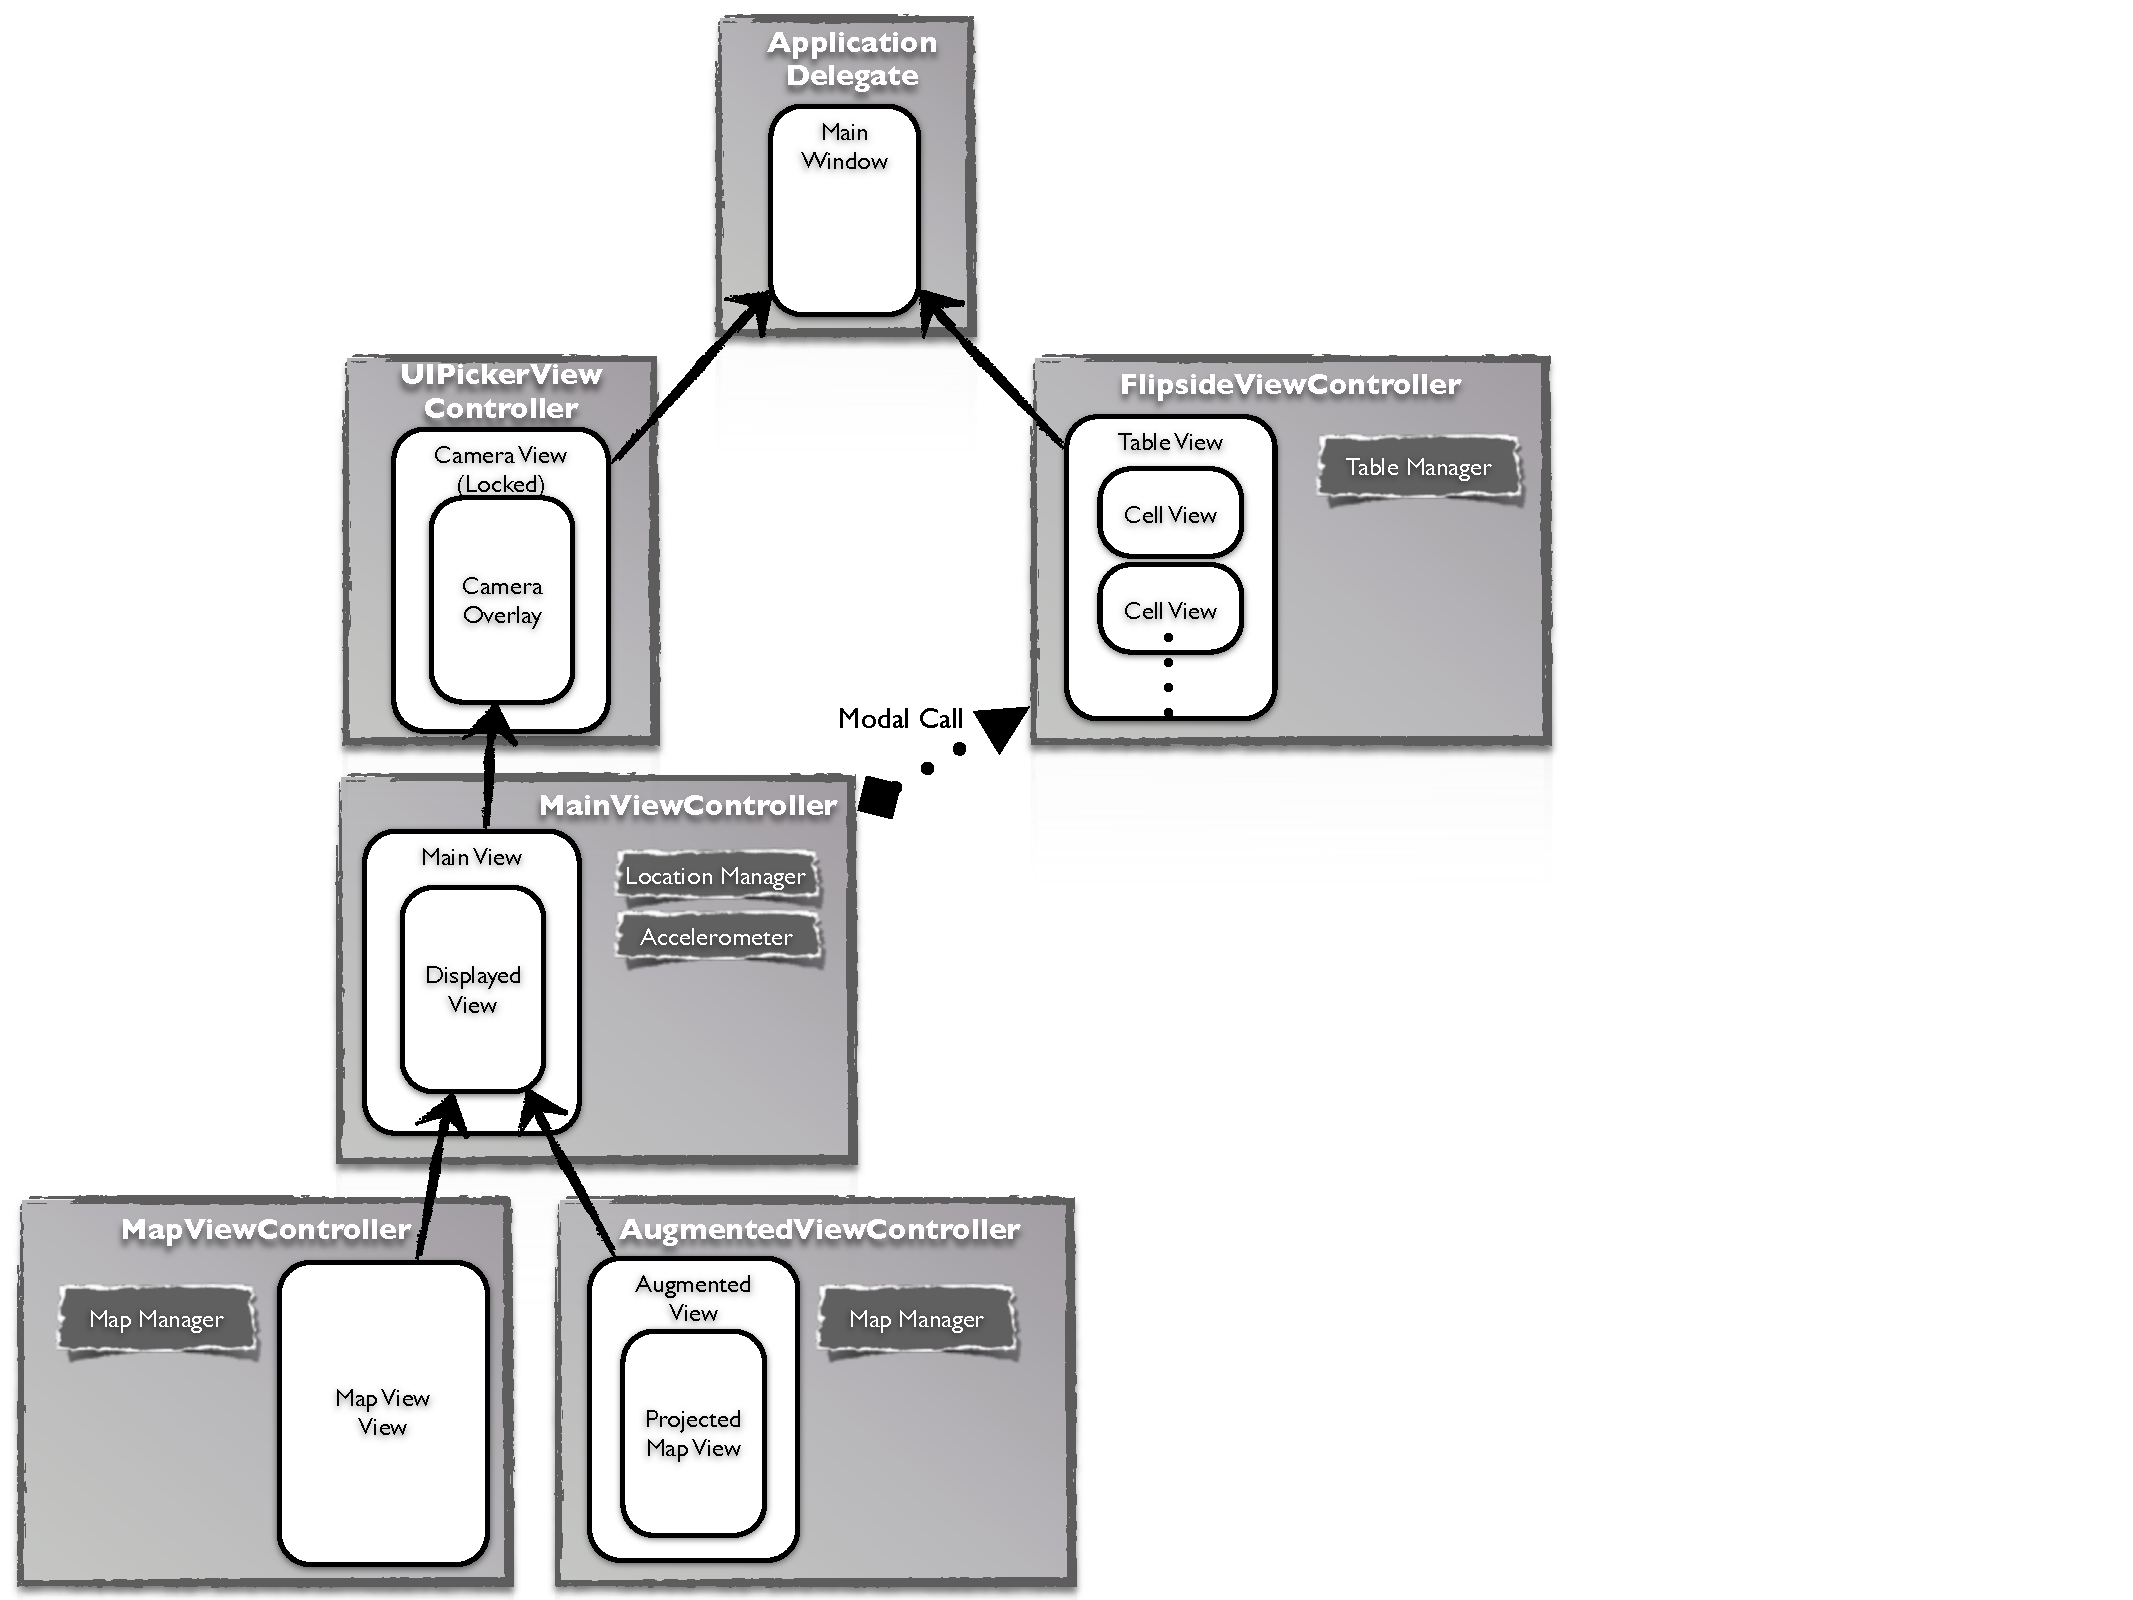
\includegraphics[scale=0.5]{pics/client_view_hierarchy}
\caption{Scheme of the View Hierarchy of the application}
\label{fig:client_view_hierarchy}
\end{figure}

\subsection{Positioning within 6 degrees of freedom}

In our application, we need to locate the camera of the iPhone within 6 degrees of freedom:

\begin{itemize}
\item{Latitude}
\item{Longitude}
\item{Altitude}
\item{Azimuth}
\item{Inclination on the X-axis}
\item{Inclination on the Z-axis}
\end{itemize}

The GPS directly gives us the Altitude, Latitude and Longitude of the user whereas the compass gives us his Azimuth.

Thanks to the 3-axis accelerometer, the inclination on the X and Z axis can be computed by the mean of simple trigonometry.

\subsection{3D Projection}

First, we project a Map on the plane defining the ground. The iPhone has an API to perform 3D projections, by the mean of layer transformations.

To apply a transform to a layer, one must provide the transform matrix corresponding to the desired projection.

In this case, the transformation will be a rotation of $\frac{\pi}{2}$ on the X-axis and a rotation corresponding to the Azimuth on the Y-Axis, followed by a translation to give depth to the view.
